\chapter{Logkorrelation in Cloud-Umgebungen}\label{02_jcorrelat}
\thispagestyle{fancy}

Im folgenden Abschnitt wird eine Forschungsarbeit der Fachhochschule Fulda 
\cite{reissmann} vorgestellt. Ziel der Forschung war und ist es, ein gut skalierendes 
System zu entwickeln um eine automatisierte Auswertung von Syslog-Meldungen in 
Cloud-Umgebungen bereit zu stellen. Aufgrund der enormen Datenmengen die in solchen 
Umgebungen anfallen kann eine Auswertung nur mittels korrelations- und 
Aggregationsverfahren geschehen. Um dieses Ziel zu erreichen kommen verschiedene 
Standards und eine Reihe von Software-Lösungen zum Einsatz.

Nachfolgend werden einige wichtige Begriffe geklärt, die Anforderungen identifiziert, die 
verwendeten Standards und die eingesetzte Software erläutert und im Weiteren Verlauf des 
Abschnitts wird anhand eines Beispiels eine Syslog-Korrelation vorgenommen.

\section{Anforderungen}\label{anforderungen}

Viele Unternehmen haben in den letzten Jahren einen großen Teil ihrer IT-Infrastruktur 
ausgelagert. Laut Analysen werden bis 2025 80 \% aller Unternehmen \cite{web_ix} 
weltweit ihre eigene Rechenzentrumsinfrastruktur abgeschaltet haben. Die wenigen Anbieter 
von Cloud-Infrastruktur stehen in Konkurrenz miteinander, daher existieren auch keine 
einheitlichen Schnittstellen um auf die Cloud-Konfigurationen zuzugreifen. Für die 
Überwachung, speziell von Sicherheitskritischen Ereignissen, stehen ebenso nur 
proprietäre Schnittstellen jedes Anbieters zur Verfügung. Aus diesem Grund soll ein 
System geschaffen werden, das die gewaltige Menge an aufkommenden Logdaten, unabhängig 
vom Anbieter, analysiert und sicherheitskritische Ereignisse unverzüglich zu 
identifiziert. Insbesondere soll das System das dynamisch sinkende und wachsende 
Syslog-Aufkommen beherrschen können. Denn durch die fluide Kostenstruktur der 
Cloud-Anbieter können schnell neue virtuelle Maschinen erstellt und entfernt werden, je 
nachdem wie viel Leistung der Kunde gerade benötigt.
Darüber hinaus sollen Meldungen auch persistent gespeichert werden, vornehmlich zur 
Erstellung von Trends und Langzeitanalysen, dabei soll der benötigte Speicherplatz so 
gering wie möglich gehalten werden.

\section{Beispielszenario}\label{szenario}

Im weiteren Verlauf dieses Kapitels soll zur detaillierteren Darstellung der 
Leistungsfähigkeit einer automatischen Syslog-Korrelation ein gängiges 
Angriffsszenario dienen. Eine \textit{ssh}-BruteForce Attacke auf eine beliebige Anzahl
an überwachten Systemen. Dabei soll genau der eine erfolgreiche Login innerhalb  der 
enormen Anzahl an erfolglosen oder ungültigen Versuchen identifiziert werden. Dieses 
recht einfache Szenario ist bei der erheblichen Anzahl an möglichen Systemen (10K+) 
manuell unmöglich zu bewerkstelligen.

\newpage
\section{JCorrelat}\label{sec_jcorrelat}

In Abbildung \ref{pic:jcorrelat} \cite[47]{reissmann} ist der schematische Aufbau von 
JCorrelat dargestellt, ein Prototyp der die Anforderungen aus Abschnitt 
\ref{anforderungen} erfüllen soll. Die hinzugefügten Nummern dienen der Übersichtlichkeit 
im weiteren Erklärungsverlauf.   

\begin{figure}[htbp]
    \caption{Aufbau von JCorrelat}
    \label{pic:jcorrelat}\vspace{0.2cm}
    \centering
    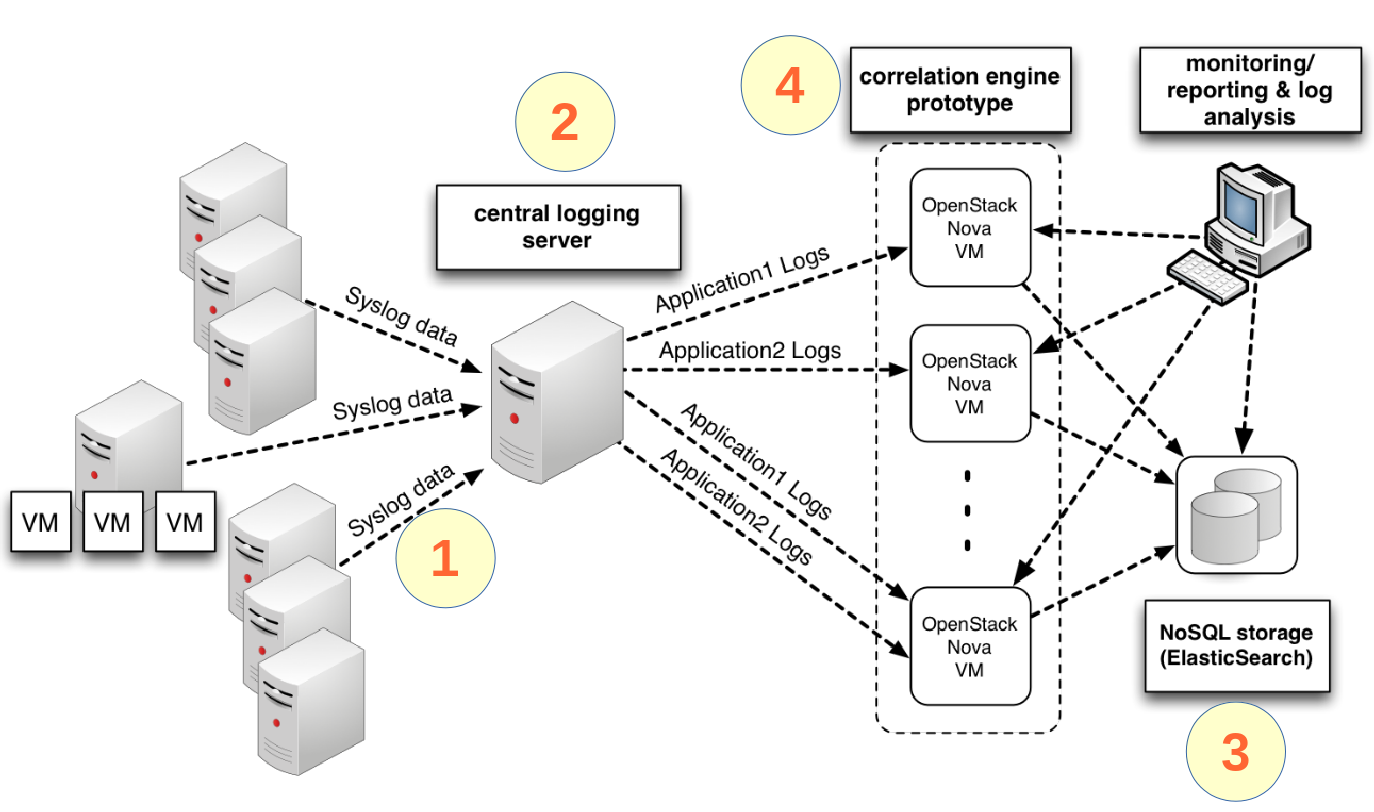
\includegraphics[scale=0.36]{img/schema-correlat}
    
\end{figure}

\subsection{Syslog-Protokoll} \label{syslog-proto}

Als Ereignisquelle und als Grundlage für neu generierte Meldungen wird das 
Syslog-Protokoll verwendet. Es ist das meist verbreitete Log-Format und wurde 
bereits in RFC 3164 standardisiert, jedoch sieht dieser Standard keine strukturierten 
Daten (\texttt{key $\Rightarrow$ value}) innerhalb einer Syslog-Nachricht vor. 
Erst mit RFC 5424 \cite{rfc5424} wurde diese Funktionalität hinzugefügt.

\begin{table}[ht]
    \caption{Aufbau RFC 5424}
    \label{table:rfc5424}\vspace{0.2cm}
    \centering{
        \renewcommand{\arraystretch}{1.3}
    \begin{tabular}{|l|c|c|}
        \hline 
        \rowcolor{gray!40} \textbf{Feld}&  \textbf{Inhalt}& \textbf{Beispiel}\\ 
        \hline
        \hline
         \multicolumn{3}{|l|}{\cellcolor{shadecolor}\textbf{HEADER}}\\
         \hline
         facility & $int \in \{0..23\}$  & $<$\textbf{16}5$>$ (\texttt{local0}) \\ 
        \hline 
        \rowcolor{green!15} severity & $ int \in \{0..7\}$  &$<$16\textbf{5}$>$  
        (\texttt{Notice})\\ 
        \hline
         timestamp & \texttt{RFC3339}  &\verb|2003-10-11T22:14:15.003Z|\\ 
        \hline 
         hostname & string  &\verb|mymachine.example.com|\\ 
        \hline 
        \rowcolor{green!15} tag &string  &\verb|evntslog|\\
        \hline
         \multicolumn{3}{|l|}{\cellcolor{shadecolor}\textbf{MESSAGE}}\\     
        \hline
         MSGID& string &\verb|ID47| \\
        \hline
        \rowcolor{green!15} structured data& key=value &\verb|eventID="1011"| \\
        \hline
         content &string&\verb|An application event log...| \\
        \hline
    \end{tabular} 
    }
\end{table}

\newpage

\begin{figure}[h]
    \caption{Beispiel RFC5424 Syslog-Meldung}
    \label{log_example}\vspace{0.2cm}
    \centering
    \begin{shaded*}
    \small{
        \begin{verbatim}
        
        
        <165> 2003-10-11T22:14:15.003Z mymachine.example.com evntslog - ID47 
        [exampleSDID@32473 iut="3" eventSource="Application" eventID="1011"] BOMAn 
        application event log entry...
        \end{verbatim}}
    \end{shaded*}
\end{figure}





Tabelle \ref{table:rfc5424} zeigt den Aufbau eines Syslog-Paketes nach RFC 5424 und 
Abbildung \ref{log_example} die dazugehörige RFC 5424 konforme Nachricht. Die für 
die weitere Verwendung wichtigsten Felder wurden grün markiert. Dazu zählt der 
Schweregrad (\textit{severity}), wobei 0 (\texttt{Emergency}) den höchsten und 7 
(\texttt{DEBUG}) 
den niedrigsten Schweregrad darstellt. Das \textit{tag}-Feld, was zum Beispiel die 
Herkunft (Programm) und die zugehörige \textit{process ID} beinhalten kann. Am 
wichtigsten ist das \textit{structured data}-Feld, welches mit beliebigen Informationen 
gefüllt werden darf.

\subsection{Konsolidierung von Syslog-Meldungen}\label{syslog-konsolidierung}

Diese Sektion erläutert Punkt \textbf{2} in Abbildung \ref{pic:jcorrelat}, es handelt 
sich um den zentralen Syslog-Server. Als Software kommt die Open Source - Lösung 
\textit{rsyslog}\footnote{\url{https://rsyslog.com}} zum Einsatz. \textit{rsyslog} ist 
RFC 5424 konform, äußerst performant und durch Module erweiterbar. Eben eines dieser 
Module kommt auch im hier vorgestellten Korrelationssystem zum Einsatz: 
\textit{liblognorm}, mittlerweile ein fester Bestandteil von \textit{rsyslog}.\\ 

Alle Applikationen senden ihre Syslog-Meldungen an diesen Server und damit auch alle 
SSH-Dienste. Somit alle Syslog-Nachrichten über einen erfolgreichen, 
fehlgeschlagenen oder ungültigen Login vor. In Abbildung \ref{ssh_example} wird 
jeweils ein Beispiel pro Fall abgebildet.

\begin{figure}[h]
    \caption{Beispiele SSH-Meldungen}
    \label{ssh_example}\vspace{0.2cm}
    \centering
    \begin{shaded*}
    \small{      
        \begin{verbatim}        


Jan 29 16:00:25 HOST sshd[2039]: Accepted password for root from 10.0.23.4 port 39110 ssh2
        
Jan 29 16:06:00 HOST sshd[2032]: Failed password for root from 10.0.23.4 port 54548 ssh2

Jan 29 16:08:39 HOST sshd[2023]: Failed password for invalid user test from 10.0.23.4 
port 57165 ssh2
\end{verbatim}}
\end{shaded*}
\end{figure}

\textit{liblognorm} ist nun in der Lage diese Meldungen auf Basis vorher definierter 
Regeln zu durchsuchen (für das konkrete Beispiel finden sich die Regeln im Anhang unter 
Abbildung \ref{app:liblognorm-rule}) und die relevanten Informationen zu extrahieren.  
Aus diesen Daten generiert liblognorm eine neue Syslog-Meldung in dem es aus den 
aufgeschlüsselten Feldern Protokoll, Nutzername, Port und Quelladresse strukturierte 
Daten bildet (Anhang: Abbildung \ref{app:liblognorm-normalisation}). Zusätzlich wird die 
neue Meldung mit einem neuen \textit{syslog-tag} names \texttt{SSHFAILURE} oder 
\texttt{SSHSUCCESS} versehen und an die Korrelationsinstanz weitergeleitet.\\

\textit{liblognorm} normalisiert und seriealisiert Daten, die aus verschiedenen Quellen 
stammen und unterschiedlich kodiert sein können zu neuen Nachrichten. Damit werden 
Redundanzen aus den Meldungen entfernt und eindeutige \textit{syslog-tags} zu schnelleren 
Identifizierung durch die Korrelationsinstanz gesetzt. 
\newpage

\subsection{Korrelation von Syslog-Meldungen}\label{syslog-korrelation}




\subsection{persistente Speicherung}\label{nosql}